% +------------------------------------------------------------------------+
% | CGAL Reference Manual:  qt_widget.tex
% +------------------------------------------------------------------------+
% | Using Qt_widget to visualize CGAL Objects
% | 
% |
% |
% | 12.12.2001  Radu Ursu
% | 
\RCSdef{\qtwidgetRev}{$Revision$}
\RCSdefDate{\qtwidgetDate}{$Date$}
% +------------------------------------------------------------------------+

\newcommand{\qt}{{\em Qt}}      %QT abbreviation

\gdef\lciIfHtmlClassLinks{\lcFalse}
\gdef\lciIfHtmlRefLinks{\lcFalse}
\gdef\lciIfHtmlLinks{\lcFalse}

\chapter{Qt\_widget}
\label{chapterQtwidget}

\ccChapterRelease{\qtwidgetRev. \ \qtwidgetDate}\\
\ccChapterAuthor{Radu Ursu}

\qt\ is a {\sc Gui} toolkit\footnote{http://www.trolltech.com} for
cross-platform application development. 

% +-----------------------------------------------------+
\section{Introduction}

In this chapter we describe a widget and some helper classes that
allow to interact with two dimensional \cgal\ objects in \qt\ based applications.

The most important class is the class \ccStyle{Qt_widget}. It provides
a drawing area and output stream operators for \cgal\ objects, as well
as zooming and panning functionality.

The \ccStyle{Qt_widget} allows to attach {\em layers}, and
it are usually layers that draw on the drawing area of the widget.
Layers can be activated and deactivated, and what you see in the drawing area
is the overlay of all attached activated layers.

The \ccStyle{Qt_widget} allows further to attach one {\em tool} at the time. 
Tools are used for entering input, and \cgal\ provides input tools for the
two-dimensional \cgal\ objects. The limitation to one tool at the time comes
from the fact that only one logical entitiy should get the focus.

Finally, we provide a {\em toolbar} for controlling the basic functionality
of the \ccStyle{Qt_widget}.

The following sections desribe the main class as well as the helper classes
in more detail and give examples that can be taken as starting points for
new applications.


\section{Qt\_widget}
\label{Qt_widget}

The class \ccStyle{Qt_widget} is derived from the \qt\ class \ccStyle{QWidget}%
\footnote{A widget is the atom of the user interface: It receives mouse, keyboard and other 
events from the window system, and paints a representation of itself on the 
screen. Every widget is rectangular, and they are sorted in a Z-order. A 
widget is clipped by its parent and by the widgets in front of it.} 
which is the base class of all \qt\ user interface objects. 


The \ccStyle{Qt_widget} provides output operators for all \cgal\ objects. There are 
operators defined for outputing : points, segments, rays, circles, triangles, 
polygons, and all type of triangulations. Also some operators are defined to 
set \ccStyle{Qt_widget}'s properties, like background and fill color, as well as line
width and point size.

As the following examples show, simple applications can be written
without the layers and tools.

\subsection{Example: Hello Segment}
The first example draws a red segment on an orange background.
\ccIncludeExampleCode{Qt_widget/Examples/hellosegment.C}

There is a severe limitation in this example: When you resize the window it is empty, as nothing is
redrawn, that is this style of programs makes only sense, if you quickly want to validate output
of a geometric computation. As in any event driven {\sc Gui} application, you have to provide 
a draw callback so that the window system can update the drawing whenever necessary. This is the topic
of the next example.

\subsection{Example: A Triangulation}

This example is slightly more involved. The user can enter points and the application
draws the Delaunay triangulation of the point set. 

\ccIncludeExampleCode{Qt_widget/basic/tutorial2/tutorial2.C}

Because the code for drawing the triangulation is put in the
\ccStyle{redraw()} function, it is drawn after, e.g., resize
operations. Note that this function first calls
\ccStyle{Qt\_widget::redraw()}. It is explained later why this must be
done.

\section{Layers}
\label{Qt_widget_layers}

In the examples from the previous section the code for drawing on the
widget was in the \ccStyle{redraw()} function. As soon as the applications are more 
involved it leads to a more modular design if one delegates the drawing task to {\em layers}. 
For example, if the application displays a Delaunay triangulation, the corresponding Voronoi diagram,
 and at the same time highlights the nearest vertex to the mouse coordinates, it makes
sense to have three independent layers. Besides better code, layers have the advantage that they
can be activated and deactivated at runtime. Finally, more modularity means a higher potential
for reuse.

A layer can be {\em attached} to a \ccc{Qt_widget}. The widget calls
the method \ccc{Qt_widget_layer::draw()} of all attached layers, in the
order that they were attached. It is a very simple rule: the last layer
attached will be drawn on top.

Also a layer can be {\em activated} and {\em deactivated}. Only active
layers are drawn, and by default a layer is activated when it gets
attached.  Note that deactivating and activating do not influence the
order of layers. You can change the order only by attaching and
detaching it.


\cgal\ provides some predefined layer classes as well as a base class
so that you can more easily write new layers.


\subsection{Example: Using A Layer for Output}
\ccIncludeExampleCode{Qt_widget/basic/tutorial3/tutorial3.C}

As you see, this example is very similar to the previous one, but
the code for drawing the triangulation is no longer in the \ccStyle{redraw()}
 function, but in a layer.

This example defines a class derived from \ccStyle{Qt_widget_layer}. In the member
function \ccStyle{draw()} it is the code for drawing the triangulation. In 
\ccStyle{My_Window} class you need an instance of \ccStyle{My_Layer} and you will 
have to attach it, if you want to see what the layer draws on the
screen.

Try to remove the line \ccStyle{attach(&v);} from the constructor to
see what happens. The application will no longer display anything. Try
to deactivate and activate the \ccStyle{layer} to see what happens.

\begin{ccAdvanced}
In the previous section I promised to explain why it is needed
Qt\_widget::redraw(); if you provide a redraw function. The
\ccStyle{Qt\_widget} paint all the layers in his \ccStyle{redraw()} member
function. If you overload this function, and you'll not call
Qt\_widget::redraw(), no layer will be shown on the screen. We
strongly encourage people to use layers instead of overloading
\ccStyle{redraw()}, even for less complex computations.
\end{ccAdvanced}


\section{Tools}
\label{Qt_widget_tools}

The main purpose of layers is to have more modular code for drawing on
the widget. Things are similar for handling input. In the previous
examples, input went through the \ccc{Qt_widget::mousePressedEvent()}
callback, which interpreted the input. In applications where you have
different kinds of input, e.g., segments and polygons in an
arrangement demo, this quickly leads to unreadable, difficult to maintain
code,  especially as typically more than one event callback is
involved. The proper way of decomposition, is delegation
of the event handling to a tool. 


A tool for \ccStyle{Qt_widget} is a class that receives events from
\ccStyle{Qt_widget} and can provide some functionality like input
objects for \ccStyle{Qt_widget} and modify already created
objects. Also some basic operations can be provided like zooming in
and out, or panning.

\cgal\ provides some predefined input tools as well as a convenience base class 
\ccStyle{Qt_widget_tool} for making it easier to develop new tools.

Only one tool at the time can be attached to a widget.

We first show how to use tools and then how they work.

\subsection{Example}

In the previous section, you could insert new points in the
triangulation by clicking on the widget. This example shows how
the same can be achieved with the help of a tool.

We attach the predefined tool \ccc{Qt_widget_get_point} to the widget,
and connect the signal emitted by the widget to the function that
handles the input.  When the user clicks with the left mouse button,
the tool creates a point and passes it to the widget. The widget then
creates a signal that gets passed to the connected slot
\ccc{My_Window::get_new_object(CGAL::Object)}.

\ccIncludeExampleCode{Qt_widget/Examples/tool.C}

The \ccStyle{Qt_widget} forwards all event callbacks to the attached tool.


\subsection{How Tools Work}

The following is an example of a tool that creates \cgal\ points when the user 
clicks the left mouse button over the widget. 
 
\begin{ccExampleCode}
namespace CGAL {

template <class R>
class Qt_widget_get_point : public Qt_widget_tool
{
public:
  typedef typename R::Point_2   Point;
  typedef typename R::FT        FT;
  
  Qt_widget_get_point(const QCursor c=QCursor(Qt::crossCursor)) :
    cursor(c) {};
  
private:
  void mousePressEvent(QMouseEvent *e)
  {
    if(e->button() == CGAL_QT_WIDGET_GET_POINT_BUTTON)
    {
      FT
        x=static_cast<FT>(widget->x_real(e->x())),
        y=static_cast<FT>(widget->y_real(e->y()));
      widget->new_object(make_object(Point(x, y)));
    }
  };
  void attaching()
  {
    oldcursor = widget->cursor();
    widget->setCursor(cursor);
  };
  
  void detaching()
  {
    widget->setCursor(oldcursor);
  };

  QCursor cursor;
}//endclass;
}//namespace CGAL
\end{ccExampleCode}

The \ccc{Qt_widget} forwards mouse and keyboard events to the attached tool.
In the above example only the \ccc{mousePressEvent} member function is overloaded.

Tools that create new \cgal\ objects, must call the member 
function \ccStyle{Qt_widget::new_object(CGAL::Object)}. The \ccStyle{Qt_widget} 
then emits the signal \ccStyle{new_cgal_object(CGAL::Object)}. This signal can be 
catched by any other object with the following connect statement:


\begin{ccExampleCode}
connect(qt_widget_ptr, SIGNAL(new_cgal_object(CGAL::Object)), 
        anyOtherObject, SLOT(anyOtherFunction(CGAL::Object)));
\end{ccExampleCode}

The first argument must be a pointer to an instance of \ccc{Qt_widget}.
In the example we connect it to \ccc{MyWindow::get_new_object(CGAL::Object)}.

\section{The Standard Toolbar}
\label{Qt_widget_standard_toolbar}

The standard toolbar includes the basic tools used for zooming and
translating.  The example further down shows how to use it in your
application.

\begin{figure}
\begin{ccTexOnly}
\begin{center}
\includegraphics{standard_toolbar.eps} 
\end{center}
\end{ccTexOnly}
\begin{ccHtmlOnly}
<CENTER>
<IMG BORDER=0 SRC="./standard_toolbar.gif"  ALIGN=center  ALT="The
standard toolbar">
</CENTER>
\end{ccHtmlOnly}
\end{figure}

\newcounter{bean}
The functionality of the toolbar is like this from the left to right:
\begin{description}
%       {Button---\Roman{bean}}{\usecounter{bean}\setlength{\rightmargin}{\leftmargin}}
        \item[Point tool:] Detach the current tool from the standard toolbar.

        \item[Zoom In:] The scales are multiplied by two keeping the same center.

        \item[Zoom Out:] The scales are divided by two keeping the same center.

        \item[Zoom In Region:] Lets you choose the center of the region where you want to zoom in. 
           The scales are multiplied by two.

        \item[Focus on the Region:] The area in the rectangle that you selected will be magnified to 
           best fit in the window.

        \item[Hand Tool:] Used for translate. Click to select the first point of translation and 
           drag to select the second point.
\end{description}

You can select a tool by clicking on a button of the standard
toolbar. To deselect the tool either you press once again the
button, or you press the arrow button that deselects the active tool,
no matter what tool it is.

\ccExample
\ccIncludeExampleCode{Qt_widget/Examples/standard_toolbar.C}

This example generates 100 points and inserts them in a Delaunay
triangulation. Using the standard toolbar you can zoom in, zoom out,
translate.

\section{Some Predefined Icons}
\label{The predefined icons}

\cgal\ provides some icons defined in some header files. This icons are
pixmaps, having the extension \ccc{.xpm}. All the icons are enumerated right
here:

\ccInclude{CGAL/IO/pixmaps/arrow.xpm}

\ccInclude{CGAL/IO/pixmaps/hand.xpm}

\ccInclude{CGAL/IO/pixmaps/holddown.xpm}

\ccInclude{CGAL/IO/pixmaps/mouse_coord.xpm}

\ccInclude{CGAL/IO/pixmaps/point.xpm}

\ccInclude{CGAL/IO/pixmaps/line.xpm}

\ccInclude{CGAL/IO/pixmaps/points.xpm}

\ccInclude{CGAL/IO/pixmaps/no_tool.xpm}

\ccInclude{CGAL/IO/pixmaps/zoom_in.xpm}

\ccInclude{CGAL/IO/pixmaps/zoom_out.xpm}

\ccInclude{CGAL/IO/pixmaps/movepoint.xpm}

\ccInclude{CGAL/IO/pixmaps/voronoi.xpm}

\ccInclude{CGAL/IO/pixmaps/triangulation.xpm}

\ccInclude{CGAL/IO/pixmaps/polygon.xpm}

To use a pixmap in your code you have to include the right file, and
to know the names of the pixmaps. The names of the pixmaps are
composed of two parts, the name of the file and the tag xpm. So for
example the arrow pixmap has the name \ccStyle{arrow\_xpm}, the line
pixmap has the name \ccStyle{line\_xpm}, and so on \ldots.  In the
tutorials and demos, almost all the pixmaps are used for the toolbar
buttons, like this:

\ccExample
\begin{ccExampleCode}
    QToolButton *get_point_but; //the toolbar button
    get_point_but =  new QToolButton(QPixmap( (const char**)point_xpm ),
                                     "Point Tool", 
                                     0, 
                                     this, 
                                     SLOT(pointtool()), 
                                     tools_toolbar, 
                                     "Point Tool");
\end{ccExampleCode}



\section{What Shall I Use?}

The previous sections presented different ways of writing \qt\ based 
applications. We recommend to use layers for the drawing task and tools
for input handling, even if you write tiny applications, because in general
they grow over time.   Layers and tools are a little bit more overhead, but 
it pays off in the long run, as you then do not have to completely
reorganize your code, to first add layers, and later add tools. 





\section{Tutorial}

In the directories \ccc{demo/Qt_widget/basic/tutorial*} we provide some examples that illustrate the widget, layers, tools, and the standard toolbar.

\subsection*{Tutorial 1}

In this tutorial you can see how can you use Qt\_widget like a stream,
for outputing \cgal\ objects.  Of course I recomend to read the tutorial
from Trolltech, that is the original Qt tutorial, but I think that you
can pass this tutorials without having strong skills of Qt
programming. Anyway, the code that belongs to Qt it is explained in
this tutorials.

The following is a typical template of how to create a window using Qt
and Qt\_widget.

\begin{ccExampleCode}
#include <CGAL/IO/Qt_widget.h>
#include <qapplication.h>

int main( int argc, char **argv )
{
    QApplication app( argc, argv );
    CGAL::Qt_widget * W = new CGAL::Qt_widget();
    app.setMainWidget( W );
    W.resize(600, 600);
    W.set_window(0, 600, 0, 600);
    W.show();

    return app.exec();
}
\end{ccExampleCode}

You'll allways need to include the header:
#include <qapplication.h>

The entry point for a typical Qt application is the function main. In
this function you should define an application object of Qt:

    QApplication app( argc, argv );

You will run the Qt application with the line:

    return app.exec();

To use Qt_widget you need an instance and tell the application to use
that instance:

    CGAL::Qt_widget *W = new CGAL::Qt_widget();
    app.setMainWidget( W );

To resize and set the scales of the window you'll use:

    W->resize(600, 600);
    W->set_window(0, 600, 0, 600);

At the end you need to show the window when the initialization have been done:

    W->show();

All the drawing code should be put betwen Qt_Widget's lock() and
unlock() functions. See the manual reference pages of Qt_widget. Doing
like this, the window will be updated only once, when Qt_widget find
the last unlock(). This way you can avoid the window flickering.

As you'll notice, this tutorial has some limitations. If you try to
resize the window you'll see that what you have been painted will
disappear. This is not a very pleasant thing but you'll see in the
next tutorial how you can solve this problem.

Applications following this approach are only usefull when you quickly
want to see how the output of a computation looks like.
\subsection*{Tutorial 2}
\subsection*{Tutorial 3}
\subsection*{Tutorial 4}
\subsection*{Tutorial 5}
\subsection*{Tutorial 6}
\subsection*{Tutorial 7}
\subsection*{Tutorial 8}

% +-----------------------------------------------------+
% EOF







